\section{Analisis Big O dan Visualisasi Kompleksitas}

Big O notation adalah notasi matematika yang digunakan untuk menggambarkan kompleksitas waktu atau ruang suatu algoritma. Notasi ini membantu kita memahami bagaimana performa algoritma berubah seiring dengan pertambahan ukuran input.

\subsection{Konsep Dasar Big O Notation}

Big O notation menggambarkan batas atas (worst case) dari pertumbuhan fungsi kompleksitas algoritma. Beberapa notasi Big O yang umum:

\begin{itemize}
  \item \textbf{O(1)} - Konstan: Waktu eksekusi tidak bergantung pada ukuran input
  \item \textbf{O(log n)} - Logaritmik: Waktu eksekusi tumbuh secara logaritmik
  \item \textbf{O(n)} - Linear: Waktu eksekusi sebanding dengan ukuran input
  \item \textbf{O(n log n)} - Linearitmaik: Kombinasi linear dan logaritmik
  \item \textbf{O(n²)} - Kuadratik: Waktu eksekusi sebanding dengan kuadrat ukuran input
\end{itemize}

\subsection{Grafik Kompleksitas Algoritma}

\begin{center}
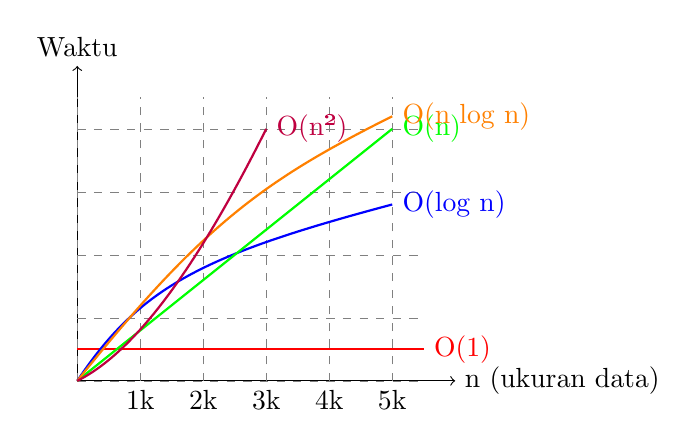
\begin{tikzpicture}[scale=0.8]
  % Axes
  \draw[->] (0,0) -- (6,0) node[right] {n (ukuran data)};
  \draw[->] (0,0) -- (0,5) node[above] {Waktu};
  
  % Grid
  \draw[gray, very thin, dashed] (0,0) grid (5.5,4.5);
  
  % O(1)
  \draw[thick, red] (0,0.5) -- (5.5,0.5) node[right] {O(1)};
  
  % O(log n)
  \draw[thick, blue] (0,0) .. controls (1,1.5) and (2,2) .. (5,2.8) node[right] {O(log n)};
  
  % O(n)
  \draw[thick, green] (0,0) -- (5,4) node[right] {O(n)};
  
  % O(n log n)
  \draw[thick, orange] (0,0) .. controls (2,2.5) and (3,3.2) .. (5,4.2) node[right] {O(n log n)};
  
  % O(n²)
  \draw[thick, purple] (0,0) .. controls (1,0.5) and (2,2) .. (3,4) node[right] {O(n²)};
  
  % Labels
  \node[below] at (1,0) {1k};
  \node[below] at (2,0) {2k};
  \node[below] at (3,0) {3k};
  \node[below] at (4,0) {4k};
  \node[below] at (5,0) {5k};
\end{tikzpicture}
\end{center}

\subsection{Tabel Kompleksitas Lengkap}

\begin{table}[htbp]
\centering
\small
\begin{tabular}{|>{\raggedright\arraybackslash}p{2.5cm}|>{\raggedright\arraybackslash}p{2cm}|>{\raggedright\arraybackslash}p{2cm}|>{\raggedright\arraybackslash}p{2cm}|>{\raggedright\arraybackslash}p{2cm}|}
\hline
\textbf{Algoritma} & \textbf{Best Case} & \textbf{Average} & \textbf{Worst Case} & \textbf{Space} \\
\hline
Bubble Sort & O(n) & O(n²) & O(n²) & O(1) \\
\hline
Selection Sort & O(n²) & O(n²) & O(n²) & O(1) \\
\hline
Linear Search & O(1) & O(n) & O(n) & O(1) \\
\hline
Binary Search & O(1) & O(log n) & O(log n) & O(1) \\
\hline
\end{tabular}
\caption{Tabel Kompleksitas Lengkap Algoritma}
\end{table}

\subsection{Analisis Performa Praktis}

\begin{table}[htbp]
\centering
\footnotesize
\begin{tabular}{|>{\raggedright\arraybackslash}p{1.8cm}|>{\raggedright\arraybackslash}p{1.4cm}|>{\raggedright\arraybackslash}p{1.4cm}|>{\raggedright\arraybackslash}p{1.7cm}|>{\raggedright\arraybackslash}p{2.3cm}|}
\hline
\textbf{n} & \textbf{O(log n)} & \textbf{O(n)} & \textbf{O(n log n)} & \textbf{O(n²)} \\
\hline
10 & 3 & 10 & 33 & 100 \\
\hline
100 & 7 & 100 & 664 & 10.000 \\
\hline
1.000 & 10 & 1.000 & 9.966 & 1.000.000 \\
\hline
10.000 & 13 & 10.000 & 132.877 & 100.000.000 \\
\hline
100.000 & 17 & 100.000 & 1.660.964 & 10.000.000.000 \\
\hline
\end{tabular}
\caption{Perbandingan Jumlah Operasi untuk Berbagai Kompleksitas}
\end{table}

\subsection{Implementasi dengan Pengukuran Waktu}

Berikut implementasi lengkap dengan pengukuran waktu eksekusi untuk membandingkan performa algoritma:

\begin{lstlisting}[language=C, caption={Program Perbandingan Performa Algoritma}]
#include <stdio.h>
#include <time.h>
#include <stdlib.h>

// Fungsi untuk mengukur waktu eksekusi
double measureTime(clock_t start, clock_t end) {
    return ((double)(end - start)) / CLOCKS_PER_SEC;
}

// Bubble Sort dengan pengukuran waktu
void bubbleSortWithTiming(int arr[], int n) {
    clock_t start = clock();
    
    int i, j, temp, swapped;
    for (i = 0; i < n-1; i++) {
        swapped = 0;
        for (j = 0; j < n-i-1; j++) {
            if (arr[j] > arr[j+1]) {
                temp = arr[j];
                arr[j] = arr[j+1];
                arr[j+1] = temp;
                swapped = 1;
            }
        }
        if (swapped == 0) break;
    }
    
    clock_t end = clock();
    printf("Bubble Sort waktu: %.6f detik\n", measureTime(start, end));
}

// Binary Search dengan pengukuran waktu
int binarySearchWithTiming(int arr[], int n, int x) {
    clock_t start = clock();
    
    int low = 0, high = n - 1;
    while (low <= high) {
        int mid = low + (high - low) / 2;
        if (arr[mid] == x) {
            clock_t end = clock();
            printf("Binary Search waktu: %.6f detik\n", measureTime(start, end));
            return mid;
        }
        if (arr[mid] < x) low = mid + 1;
        else high = mid - 1;
    }
    
    clock_t end = clock();
    printf("Binary Search waktu: %.6f detik\n", measureTime(start, end));
    return -1;
}

int main() {
    const int SIZE = 10000;
    int arr[SIZE];
    
    // Generate random data
    srand(time(NULL));
    for (int i = 0; i < SIZE; i++) {
        arr[i] = rand() % 10000;
    }
    
    printf("Mengurutkan %d elemen...\n", SIZE);
    bubbleSortWithTiming(arr, SIZE);
    
    printf("Mencari elemen...\n");
    int result = binarySearchWithTiming(arr, SIZE, 5000);
    
    if (result != -1) {
        printf("Elemen ditemukan pada indeks %d\n", result);
    } else {
        printf("Elemen tidak ditemukan\n");
    }
    
    return 0;
}
\end{lstlisting}

\subsection{Tips Optimasi Algoritma}

\begin{itemize}
  \item \textbf{Pilih algoritma yang tepat:} Sesuaikan dengan karakteristik data
  \item \textbf{Pertimbangkan ukuran data:} Untuk data kecil, algoritma sederhana mungkin lebih cepat
  \item \textbf{Analisis trade-off:} Memory vs speed, simplicity vs efficiency
  \item \textbf{Profile kode:} Ukur performa aktual untuk identifikasi bottleneck
  \item \textbf{Gunakan algoritma yang sudah teruji:} Library function biasanya sudah dioptimasi
\end{itemize}

Pemahaman Big O notation sangat penting untuk mengembangkan algoritma yang efisien dan scalable, terutama untuk aplikasi yang menangani data dalam jumlah besar.
